\documentclass{article}
\usepackage[utf8]{inputenc}
\usepackage[swedish]{babel}
\usepackage{url}
\usepackage{minted}
\usepackage{graphicx}
\usepackage{float}

\title{Introduktionslabb}
\author{Fredrik Lundborg}
\date{\today}

\begin{document}

\maketitle

\section*{Introduktion}
Tanken med denna labben är att ni ska ladda ner den nödvändiga mjukvaran för att kunna arbeta med era Raspberry Picos W. Ni ska sedan skriva kod för att ansluta till internet via Wifi samt blinka med en LED.

\section*{Mjukvara}
Vår mikrokontroller kommer inte med förinstallerad programvara, utan det är något som vi måste förse den med. Detta är dock en enkel process, håll inne knappen som lyder BOOTSEL på Picon och koppla in den med en usb-kabel till datorn, Picon kommer nu komma upp i datorn som ett minne, det vi behöver göra är att ladda ner den senaste \texttt{uf2}-filen från MicroPythons Hemsida \url{https://micropython.org/download/rp2-pico-w/}. Kopiera sedan över denna fil till Picon (drag and drop till pico-minnet). Koppla sedan ut mikrokontrollern och koppla in igen utan att hålla inne BOOTSEL.

\section*{Thonny}
Se till att ha senaste versionen av Python installerad på datorn. Gå sedan till Thonny's hemsida \url{http://www.thonny.org} och ladda ner programmet. Installera sedan filen som laddas ner. Väl inne i Thonny, klicka på \texttt{Run} $\rightarrow$ \texttt{Select Interpreter}, välj MicroPython (Raspberry Pi Pico) som interpreter och välj sedan den Port som din Raspberry Pi Pico inkopplad till, det skall stå något om seriell USB enhet, se bild \ref{fig:thonny}.

\begin{figure}[H]
    \centering
    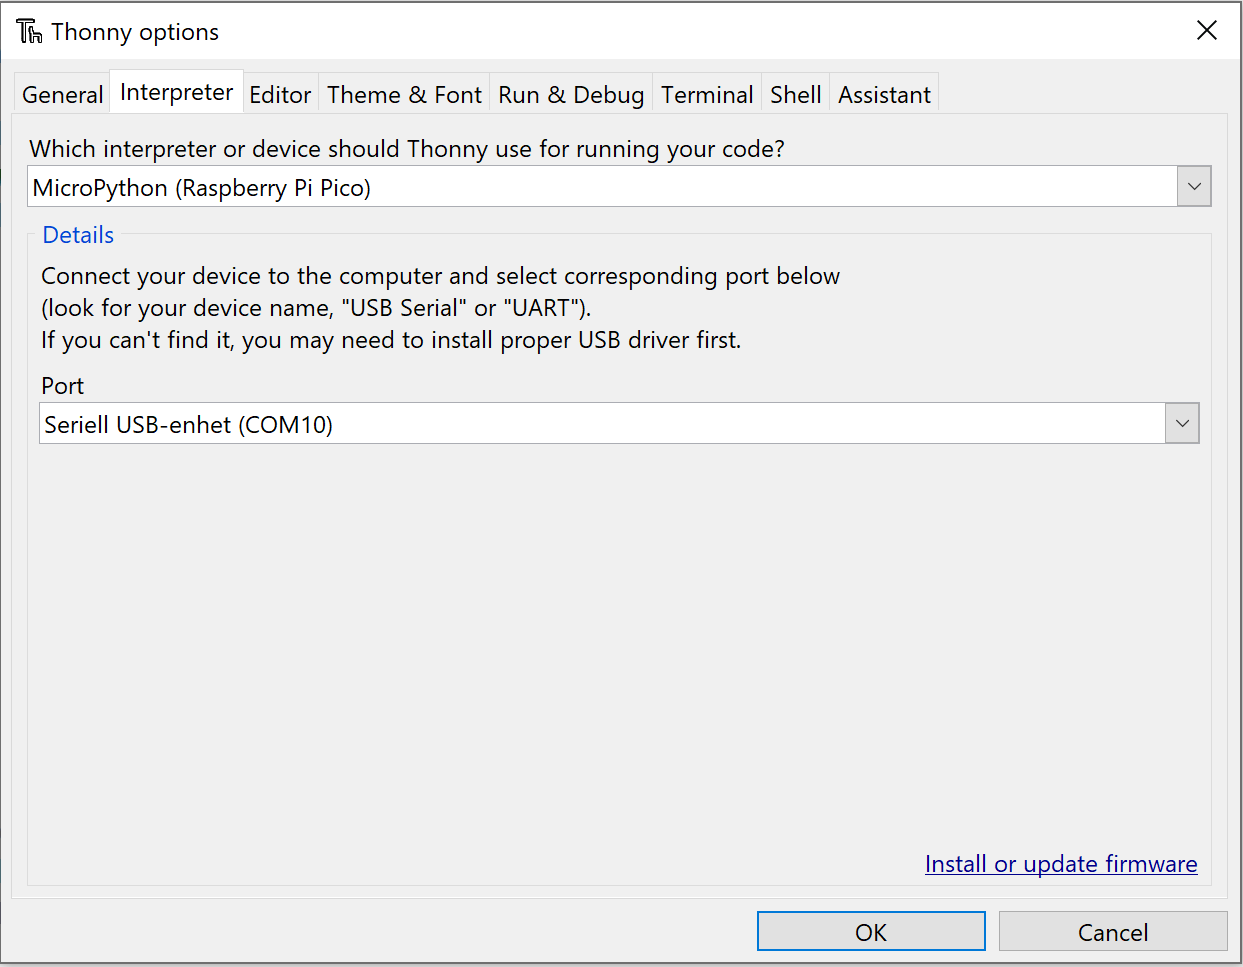
\includegraphics[scale = 0.7]{thonny.png}
    \caption{Exempel på vilken port som väljs.}
    \label{fig:thonny}
\end{figure}

\section*{Uppgifter}
\subsection*{Koppla upp till wifi}
Eran första uppgift är att koppla upp er Pico till wifi. Vi rekommenderar att ni använder eget wifi för detta, är ni på plats i skolan så fungerar det bra att dela internet från mobilen. Något som är värt att tänka på är att Raspberry Picos ej funkar med 5 GHz wifi!

För att komma åt wifi funktionerna på era Picos så måste ni i eran kod importera \texttt{network} biblioteket.
Som regel när man skriver kod med känslig data, detta fall wifi lösenord och wifi namn, så brukar man vilja göra en separat fil som sedan importeras in i era main filer. Typen av wifi anslutning vi vill ha under denna kursen är en station. När ni anslutit så visa eran anslutning genom att printa er \texttt{ifconfig}.

För relativt detaljerade instruktioner rekommenderas guiden på Tom's Hardware, både för en minimal uppkoppling:
\url{https://www.tomshardware.com/how-to/connect-raspberry-pi-pico-w-to-the-internet}

Och för en något längre version med webbserver (samt info om hur du printar ut din \texttt{ifconfig}):\\
\url{https://www.tomshardware.com/how-to/raspberry-pi-pico-w-web-server}

Observera att du behöver inte göra en webbserver (men du får givetvis), men kommandon för att få ut \texttt{ifconfig} finns där. Kommandot (eller programmet) \texttt{ifconfig} håller reda på en dators (eller annan enhets) nätverksuppkopplingar. Det kommer från en förkortning från \texttt{interface config}.
\subsection*{LEDS}
I andra delen av den här labben vill vi att ni skriver en enkel kod som får en LED att blinka. För det så behöver ni först koppla in er LED på en utav Picons GPIO (General Purpose Input/Output), se figur \ref{fig:pico}. Och sedan det andra benet till ground. I de flesta fall vill vi även använda en resistor, men Picon har inte förmågan att leverera tillräckligt med ström för att skada våra LEDS.

För att komma åt era pins behöver ni i eran kod importera \texttt{Pin} från biblioteket \texttt{machine}. För att sedan deklarera en pin att styra kan ni använda koden:

\begin{minted}{python}
from machine import Pin
led1 = Pin(13,Pin.OUT)   
\end{minted}
Notera här att 13 motsvarar GPIO 13, \emph{inte} den trettonde inkopplingspinen på Picon. I Thonny finns en texteditor som behöver användas för att skriva koden som skall köras på Picon, när du sparar skall du välj att spara ditt program på Picon.

Skriv en kod som får er lampa att blinka med en frekvens på en blinkning per sekund.
För att styra utgången tar \texttt{led1} argument, dvs skriver du \texttt{led1(1)} bör lysdioden tändas och skriver du \texttt{led1(0)} slocknar den. Modulen \texttt{time} innehåller en funktion som heter \texttt{sleep} som tar som argument antal sekunder programmet skall vänta innan det går vidare. Importera funktionen \texttt{sleep} på följande sätt:
\mint{python}|from time import sleep|
För att repetera programraderna kan en \texttt{while}-loop användas, ett (lite fuskigt) sätt är att köra en evig loop, var noga med att det som är inne i loopen måste stå fyra blanksteg in på raden (Python använder inte parenteser). Tex:
\begin{minted}{python}
while True:
    do_something
\end{minted}
\begin{figure}[h]
    \centering
    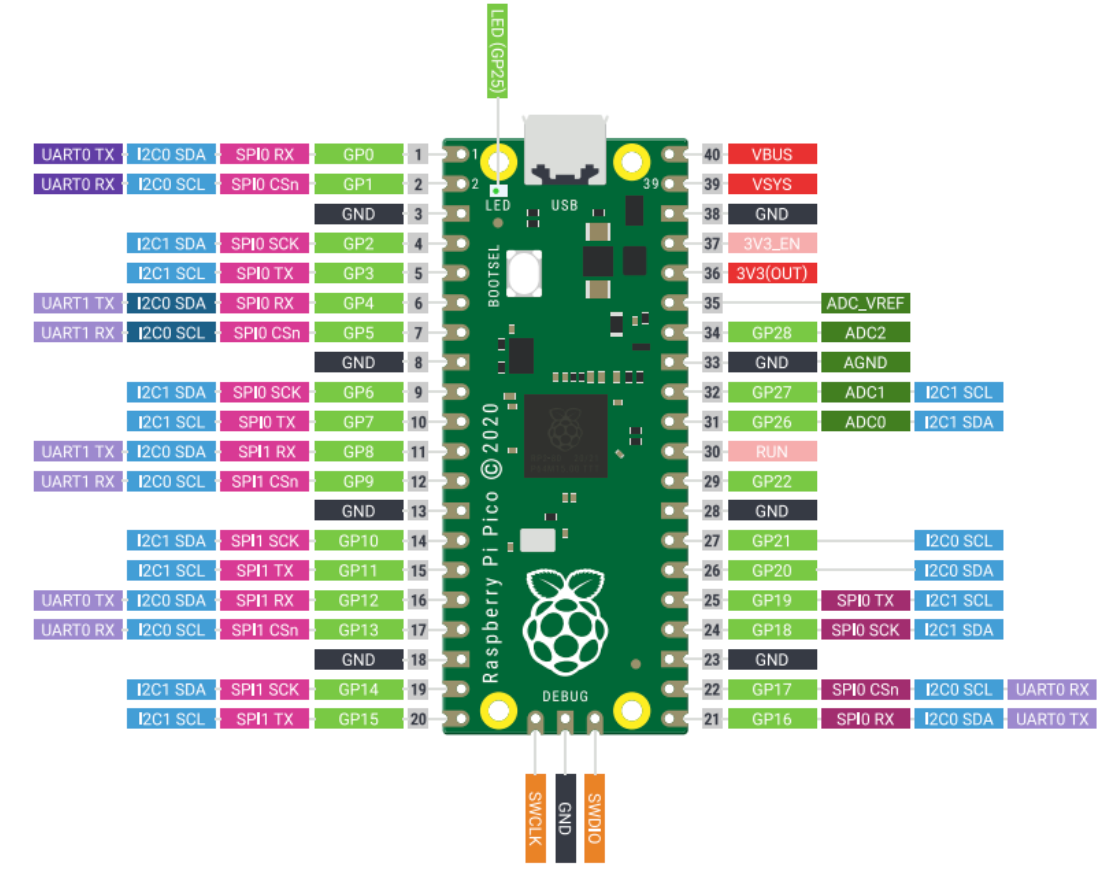
\includegraphics[scale=0.5]{picopinout.png}
    \caption{Pico Pinout.}
    \label{fig:pico}
\end{figure}
\end{document}
